\documentclass{fancyslides} 
\usepackage[utf8]{inputenc}
\usepackage{times}
\usepackage{algorithm2e}
\usepackage{listings}
\usepackage{hyperref}


%%% Beamer settings (do not change)
\usetheme{default} 
\setbeamertemplate{navigation symbols}{} %no navigation symbols
\setbeamercolor{structure}{fg=\yourowntexcol} 
\setbeamercolor{normal text}{fg=\yourowntexcol} 



%%%%%%%%%%%%%%%%%%%%%%%%%
%%% CUSTOMISATIONS %%%%%%
%%%%%%%%%%%%%%%%%%%%%%%%%

% THE FOLLOWING COLOURS ARE PREDEFINED IN THE CLASS
%bi -- WHITE
%cz -- BLACK
%sz -- GRAY
%nieb -- BLUE
%ziel -- GREEN
%pom -- ORANGE
%% YOU CAN DEFINE YOUR OWN COLOUR TO USE HERE. SEE MAN.PDF


%%%% SLIDE ELEMENTS
\newcommand{\structureopacity}{0.75} %opacity for the structure elements (boxes and dots)
\newcommand{\strcolor}{ziel} %elements colour (predefined nieb; pom; ziel)

%%%% TEXT COLOUR
\newcommand{\yourowntexcol}{bi}
\newcommand{\stext}[1]{{\color{black}#1}}
\newcommand{\ctext}[1]{{\ttfamily#1}}



%%%%%%%%%%%%%%%%%%%%%%%%%
%%% TITLE SLIDE DATA %%%%
%%%%%%%%%%%%%%%%%%%%%%%%%
\newcommand{\titlephrase}{Mesh Processing with OpenMesh and C++}
\newcommand{\name}{Alexandre Kaspar}
\newcommand{\affil}{EPFL / MIT}
\newcommand{\email}{akaspar@mit.edu}





\begin{document}

%\fontencoding{T1}
%\fontfamily{serif}
%\fontseries{m}
%\fontshape{it}
%\fontsize{12}{15}
%\selectfont

\lstset{
	language=C++,
    basicstyle=\color{black}\ttfamily,
    keywordstyle=\color{blue},
    identifierstyle=\color{gray!50!black},
    stringstyle=\color{green!50!black},
    commentstyle=\color{gray}\ttfamily\textit,
    morecomment=[l][\color{magenta}]{\#},
    numbers=left,
    numberstyle=\ttfamily,
    numbersep=10pt
}

\startingslide %this generates titlepage from the data above


\fbckg{backgrounds/code2}
\begin{frame}
\pointedsl{C++}
\end{frame}

% based on http://ocw.mit.edu/courses/electrical-engineering-and-computer-science/6-096-introduction-to-c-january-iap-2011/index.htm

\setbeamercolor{frametitle}{fg=gray}
\fbckg{backgrounds/code2}
\begin{frame}
\frametitle{History}
\itemized{
	\item Created in 1979 by Bjarne Stroustrup
	\item Extension of C
}
\end{frame}


\fbckg{backgrounds/blank2}
\begin{frame}
\frametitle{Compiling}
\begin{center}
	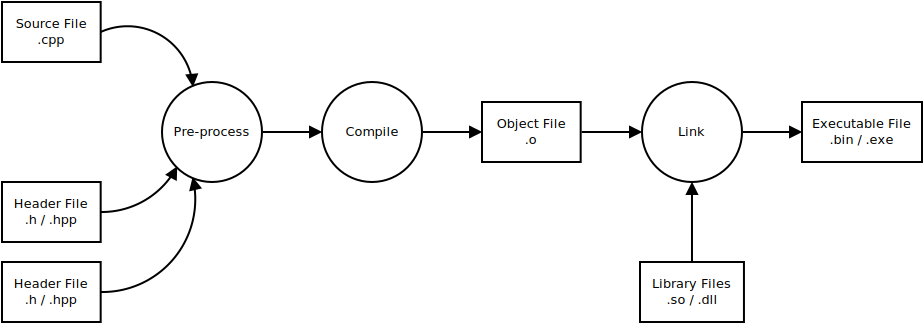
\includegraphics[width=0.97\textwidth]{figures/compiler}
	\end{center}
\misc{
	The \emph{compiler} translates source files (.cpp) into object files (.o).
	
	The \emph{linker} provides information to link object files (.o) together with libraries, producing an executable file (.exe).
}
\end{frame}






\begin{frame}[fragile]
\frametitle{Hello World}
\begin{lstlisting}
#include<stdio.h>
#include<iostream>
// A comment
int main(int argc, char **argv){
    std::cout << "Hello world!" << std::endl;
    return 0;
}
\end{lstlisting}
\misc{
	Outputs "Hello world" in console and exits.
}
\end{frame}




\begin{frame}[fragile]
\frametitle{Pre-processor instructions}
\begin{lstlisting}
#include<stdio.h>
#include<iostream>
\end{lstlisting}
\misc{
	Lines starting with a `\#' (pound) are instructions parsed by the \emph{pre-processor} such as
	\begin{itemize}
	\item \textbf{\#include} specifies a file to be included at this line.
	\item \textbf{\#if, \#ifdef, \#endif} conditionally uses a block of code.
	\item \textbf{\#define} creates an alias for an expression.
	\end{itemize}
}
\end{frame}





\begin{frame}[fragile]
\frametitle{Comments}
\begin{lstlisting}[firstnumber=3]
// A comment (up to the end of the line)
\end{lstlisting}
\stext{or}
\begin{lstlisting}[firstnumber=3]
/* A comment 
possibly spanning
multiple lines */
\end{lstlisting}
\misc{
	are comments, which both the compiler ignores.
}
\end{frame}





\begin{frame}[fragile]
\frametitle{Main function}
\begin{lstlisting}[firstnumber=4]
int main(int argc, char **argv){
    ...
    return 0;
}
\end{lstlisting}
\misc{
	defines a function named \ctext{main} which
	\begin{itemize}
		\item takes two arguments \ctext{argc} and \ctext{argv},
		\item returns an integer value (\ctext{int} in front).
	\end{itemize}
}
\end{frame}

\begin{frame}[fragile]
\frametitle{Main function}
\begin{lstlisting}[firstnumber=4]
int main(int argc, char **argv){
    ...
    return 0;
}
\end{lstlisting}
\misc{
	The \ctext{main} function is the one which is called when the program starts, with
	\begin{itemize}
		\item \ctext{argc}, the number of arguments
		\item \ctext{argv}, the arguments (array of strings)
	\end{itemize}
	and returns an integer code ($0=$ success).
}
\end{frame}






\fbckg{backgrounds/blank2}
\begin{frame}
  \thankyou   %%%% ending slide with thank you notice
\end{frame}





\fbckg{backgrounds/blank}
\begin{frame}
\sources{
\includegraphics[height=1em]{figures/C++-logo} \ \href{http://ocw.mit.edu/courses/electrical-engineering-and-computer-science/6-096-introduction-to-c-january-iap-2011/index.htm}{Introduction to C++,  MIT OpenCourseWare}\\
\includegraphics[width=0.5cm]{figures/C++-logo} \ flickr/apsmuseum
}
\end{frame}


\end{document}